%% ----------------------------------------------------------------------------
% BIWI SA/MA thesis template
%
% Created 09/29/2006 by Andreas Ess
% Extended 13/02/2009 by Jan Lesniak - jlesniak@vision.ee.ethz.ch
%% ----------------------------------------------------------------------------

% Give an introduction to the topic you have worked on:
% 
% \begin{itemize}
%  \item \textit{What is the rationale for your work?} Give a sufficient description of the problem, e.g. with a general description of the problem setting, narrowing down to the particular problem you have been working on in your thesis. Allow the reader to understand the problem setting. 
%  \item \textit{What is the scope of your work?} Given the above background, state briefly the focus of the work, what and how you did.
%  \item \textit{How is your thesis organized?} It helps the reader to pick the interesting points by providing a small text or graph which outlines the organization of the thesis. The structure given in this document shows how the general structuring shall look like. However, you may fuse chapters or change their names according to the requirements of your thesis.
% \end{itemize}

\chapter{Introduction}
With the increase of computational power the field of computer vision has made huge leaps forward in recent years. The integration of machine learning techniques and especially the introduction of deep Convolutional Neural Networks (CNN) allowed for unparalleled performance on both classification and detection tasks~\cite{krizhevsky2012}. Convolutional neural network do not only automate feature selection and classification, but also allow for automatic feature design, which has been a complicated topic in computer vision research over the years. Neural networks are very flexible and have the capability to learn every type of function. However with networks typically requiring several millions of parameters, those networks need large labeled datasets to prevent overfitting and to learn powerful generalizable models.

Nowadays datasets like Imagenet provide millions of labeled images in over thousands of categories~\cite{deng2009}, overcoming earlier shortcomings of smaller datasets. Efforts to scale these methods to billions of images are however hampered by the expense of human annotation required~\cite{doersch2015}, limiting possibilities for improvements in the future. The costly and time-consuming process of manual annotation harms the scalability to new problem domains, especially for tasks involving more complex data (for example videos and measurements from 3D sensors) and tasks requiring human expertise~\cite{lee2017,fernando2017}. In this context it would be legitimate to ask: do we really need strong-supervision from so many images to train those CNNs~\cite{wang2015}?

Unfortunately, despite decades of sustained effort, unsupervised learning have not yet reached the level to allow it to extract useful information from large collection of full-size images~\cite{doersch2015}. Humans, however, excel in inferring 3D structure to develop a strong belief of structure also in short timescales, while receiving only limited semantic supervision. One hypothesis of the reason humans perform so well in this task is that we develop a rich structural understanding of the world through past visual experience and creating consistent modeling of our observations~\cite{zhou2017}. One can conclude that context is an important factor in the development of knowledge, which subsequently leads to the concept of self-supervised learning.

\begin{figure}[t]
\centering
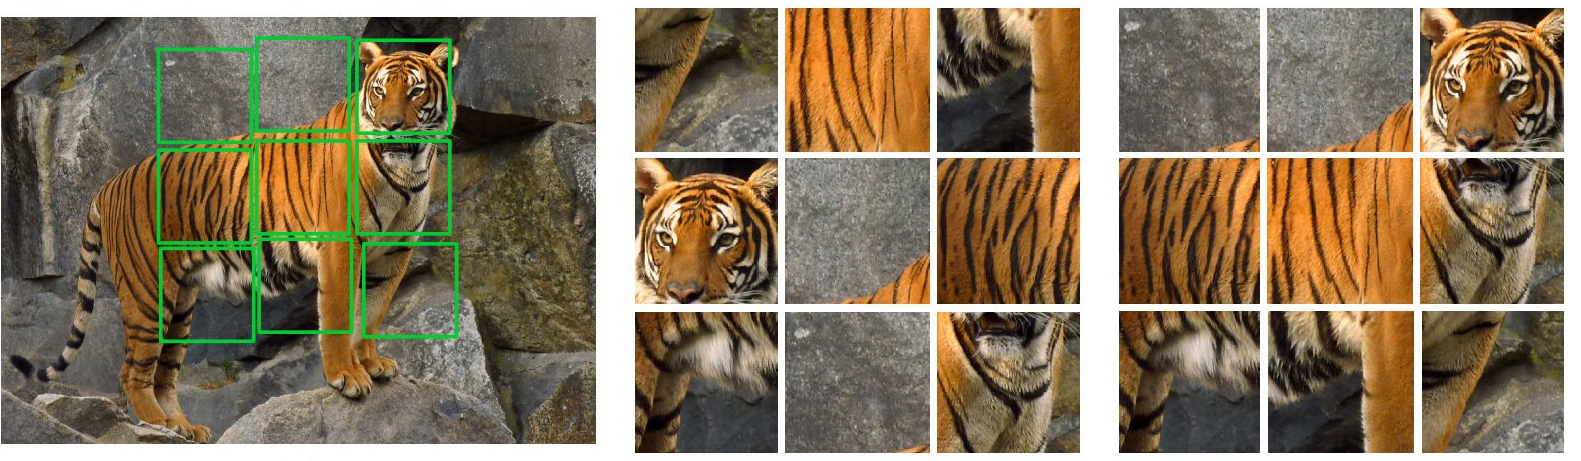
\includegraphics[width=\textwidth]{images/jigsaw_puzzle.png}
\caption{Example of a self-supervised task explored by Noorozi et al.\cite{noroozi2016} to let a neural network solve a jigsaw puzzle. Tiles (green) are extracted from the image and a puzzle is obtained after shuffling the tiles. The permutation index is used as label for the CNN to estimate. Figure is reproduced from \cite{noroozi2016}.}
\label{fig:jigsaw}
\end{figure}

Self-supervised learning involves the use of 'free' supervision available by exploiting intrinsic structure of data for training neural networks. Self-supervised learning techniques can exploit reward signals from for example spatial coherence by learning the correct location of patches~\cite{doersch2015, noroozi2016} as shown in more detail in Figure \ref{fig:jigsaw}. Alternatively temporal coherence can be used, for example by learning to order frames in videos~\cite{misra2016, lee2017}, the task also studied in this work. Many self-supervised tasks are interesting in their own right, but their direct functional use is usually limited to very specialized domains (the network to order frames could for example help in making videos from separate pictures, but usually available accurate timing information makes this task much easier).

The tasks remain however very interesting, to inspect the strength of various input features, to investigate the semantic understanding of the network on different problems, as well as indirectly in other tasks by generalizing the network to broader applications. By using transfer learning the performance on a related supervised task as object detection can be improved, as the networks hopefully already learns similar visual patterns with the self-supervised task~\cite{raina2007}. In the framework of CNNs this optimization procedure is usually referred to a 'fine-tuning', having the goal of reaching similar classification performance with much less supervision by exploiting the earlier learning.
%Because the supervised task does not have to be trained from scratch less training data is required and therefore less manual labeling. 

In this work we hypothesize that autonomous driving poses an interesting application for self-supervised learning. Self-driving cars have opened a field of research that has recently seen a huge interest both from a commercial perspective as well as in the research community. Recent studies had a heavy focus in the direction of computer vision, with detection of objects as cars, pedestrians and signs being a major component in allowing to drive autonomously. The application of convolutional neural networks has achieved huge success in improving object detection\cite{bojarski2016end}, but suffers again from the requirement of huge annotated datasets for sufficient performance. Various datasets like the KITTI~\cite{geiger2012} and the Oxford Robotcar~\cite{maddern2017} dataset contain driving videos with cameras from various perspectives, combined with high-quality lidar measurements, precise GPS tagging and accurate timing captured by the various sensors. These datasets therefore have extensive intrinsic structure and should thus be an excellent source for self-supervised learning with strong context signals. 

In the past computer vision research has primarily focused on camera images, however lidar in particular is another rich extra source of information that could be exploited for learning. Especially in a self-supervised context, this line of approach has not been actively researched. While the usage of lidar as individual feature map is interesting, especially combining networks with multiple input signals is expected to be a promising approach. A self-supervised task serves as an interesting possibility to evaluate the strength of features from a lidar, because it is does not require any particular labeling.

\section{Focus of this Work}
This project tries to take advantage of the free data in datasets captured from cars aimed at autonomous driving. More specifically the KITTI dataset~\cite{geiger2012} has been chosen for this purpose. All the labels in this dataset are not used, and instead self-supervising techniques are explored to train a network. As the data from autonomous driving datasets is mostly video data, it makes naturally sense to choose an order-prediction task to investigate the learning of temporal coherence using various input sources.

The project has two main goals:
\begin{enumerate}
\item Explore a self-supervised order-prediction task with different network variations and attempt to develop an interpretation of the semantic understanding of the performance of the network, to understand the feasibility of the network on other related tasks.
\item Study the strength of different feature maps extracted from the sensors, a novel direction of research in the area of self-supervised learning. In this respect both camera images and several feature maps extracted from lidar are used to investigate the strength of different features. Furthermore experiments to combine the camera and lidar features at different depths of the CNN are carried out, to study the way the input sources can enrich each other
\end{enumerate}.

\section{Thesis Organization}
The remainder of this thesis is divided in three main chapters. In Chapter \ref{ch:related_work} previous work is presented, to show related research in the field of self-supervised learning and related strategies. Also various techniques to process 3D lidar signals to allow them to be fed to neural networks are introduced. 

In Chapter \ref{ch:approach_implementation} the general approach and implementation are discussed with the preprocessing, data sampling and the various feature maps studied in this work. Also the overall implementation of various components in the Caffe framework are provided in more detail. 

Then the actual experiments and results are presented in \ref{ch:experimentsandresults}, containing the performance of the neural network on various variations of the network with different input features and different combinations of these. Moreover, results on some additional interesting experiments are provided.

Hereafter a discussion about the performance of the CNN, it strength and weaknesses on different section and an investigation of the features the network learns follows in Chapter \ref{ch:discussion}. Finally in Chapter \ref{ch:conclusion} the work is concluded and several possibilities for future research are suggested. 

In the following Appendix \ref{app:implementation_details} the most important implementation details are given to allow to reproduce this work and to use the developed tools for new experiments. In the next Appendix \ref{app:additional_visualizations} some additional visualizations are provided not shown elsewhere in this thesis.
